\subsection{Estándares existentes}

    El estándar internacional IEC 61508 define un conjunto de estrategias y buenas prácticas para ser aplicadas en el diseño de sistemas críticos, eléctricos y electrónicos, en diversas industrias. Entre las industrias alcanzadas encontramos la industria nuclear, la industria automotriz y la industria ferroviaria, como se puede visualizar en la Figura \ref{fig:IEC_61508}.

    \begin{figure}[h]
        \centering
        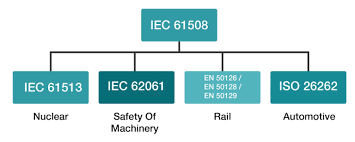
\includegraphics[width=1\textwidth]{Figuras/IEC61508.png}
        \centering\caption{Estándar IEC 61508.}
        \label{fig:IEC_61508}
    \end{figure}

    Dentro del universo de estándares ferroviarias, nos enfocaremos principalmente en tres de ellas: EN-50126, EN-50128 y EN-50129. Una falla en un sistema crítico puede poner en peligro cientos de vidas humanas y/o dañar la costosa infraestructura del sistema. Es por eso que los sistemas de enclavamiento deben cumplir los estrictos parámetros de fiabilidad, disponibilidad, mantenibilidad y seguridad (RAMS, del inglés Reliability, Availability, Mantenibility and Safety), durante todo el ciclo de vida definido en el estándar EN-50126.

    Adicionalmente, el estándar EN-50126 define el nivel de integridad de seguridad (SIL, del inglés Safety Integrity Level). Este parámetro no es del sistema en su conjunto, sino que se asocia a las funciones de seguridad asociadas al sistema, pudiendo tener diferentes SILs dentro de un mismo dispositivo. Se definen 4 SIls, siendo el nivel es el mas alto y, por lo tanto, el que tolera menos fallas. Aunque existen diversos factores que impactan en la determinación del SIL, podemos tomar como referencia el criterio definido en la Tabla \ref{Tab:tabla_SIL} en función de la probabilidad de fallas por hora (PFH) del sistema funcionando de forma continua.

    \begin{table}[!h]
        {
        \caption{Asignación del SIL en función de la Probabilidad de Fallas por Hora (PFH).}
        \label{Tab:tabla_SIL}
        \centering
        %\small
            %\centering
            \begin{center}
            \resizebox{0.5\textwidth}{!}{
            \begin{tabular}{ c | c c c c c }
                %\hline	
                   SIL & & & & &  \\	
                \hline
                   4 & 10-8 & \multirow{4}{*}{>} & \multirow{4}{*}{PFH} & \multirow{4}{*}{>} & 10-9 \\
                   3 & 10-7 & &  & & 10-8 \\
                   2 & 10-6 & &  & & 10-7 \\
                   1 & 10-5 & &  & & 10-6 \\
                %\hline
            \end{tabular}
            }
            \end{center}
        }    
    \end{table}

    El estándar EN-50128 establece las buenas prácticas, metodologías y técnicas aplicables en el área de software para lograr el SIL objetivo. Algunas de estas técnicas pueden ser obligatorias, altamente recomendadas, recomendadas, desaconsejadas o prohibidas. En algunos casos es obligatorio elegir entre diferentes combinaciones de metodologías optativas. Podemos encontrar entre estas: evitar el uso de punteros, elegir un lenguaje fuertemente tipado, modularizar el código, prohibición de usar memoria dinámica, etc. Este estándar solo se aplica si el sistema incluye un microprocesador con software embebido.

    El estándar EN-50129 es el equivalente en hardware al estándar EN-50128. Las metodologías definidas en EN-50129 se centran en la elección de componentes electrónicos, compatibilidad electromagnética y dos conceptos fundamentales: redundancia y diversidad.

    La redundancia en sistemas críticos se define mediante la abreviatura NooM (N de M, del inglés, N out of M). Donde M representa la cantidad de módulos de medición/decisión que posee el sistema y N la cantidad de módulos que deben funcionar correctamente para que el sistema opere normalmente [REF]. En la Figura \ref{fig:redundancia} se puede apreciar un sistema con redundancia 2oo3, en el cual se tendrá una salida correcta siempre que se tenga a lo sumo un fallo por vez, no acumulativo. El sistema determina, mediante votación, la respuesta correcta del sistema.

    \begin{figure}[h]
        \centering
        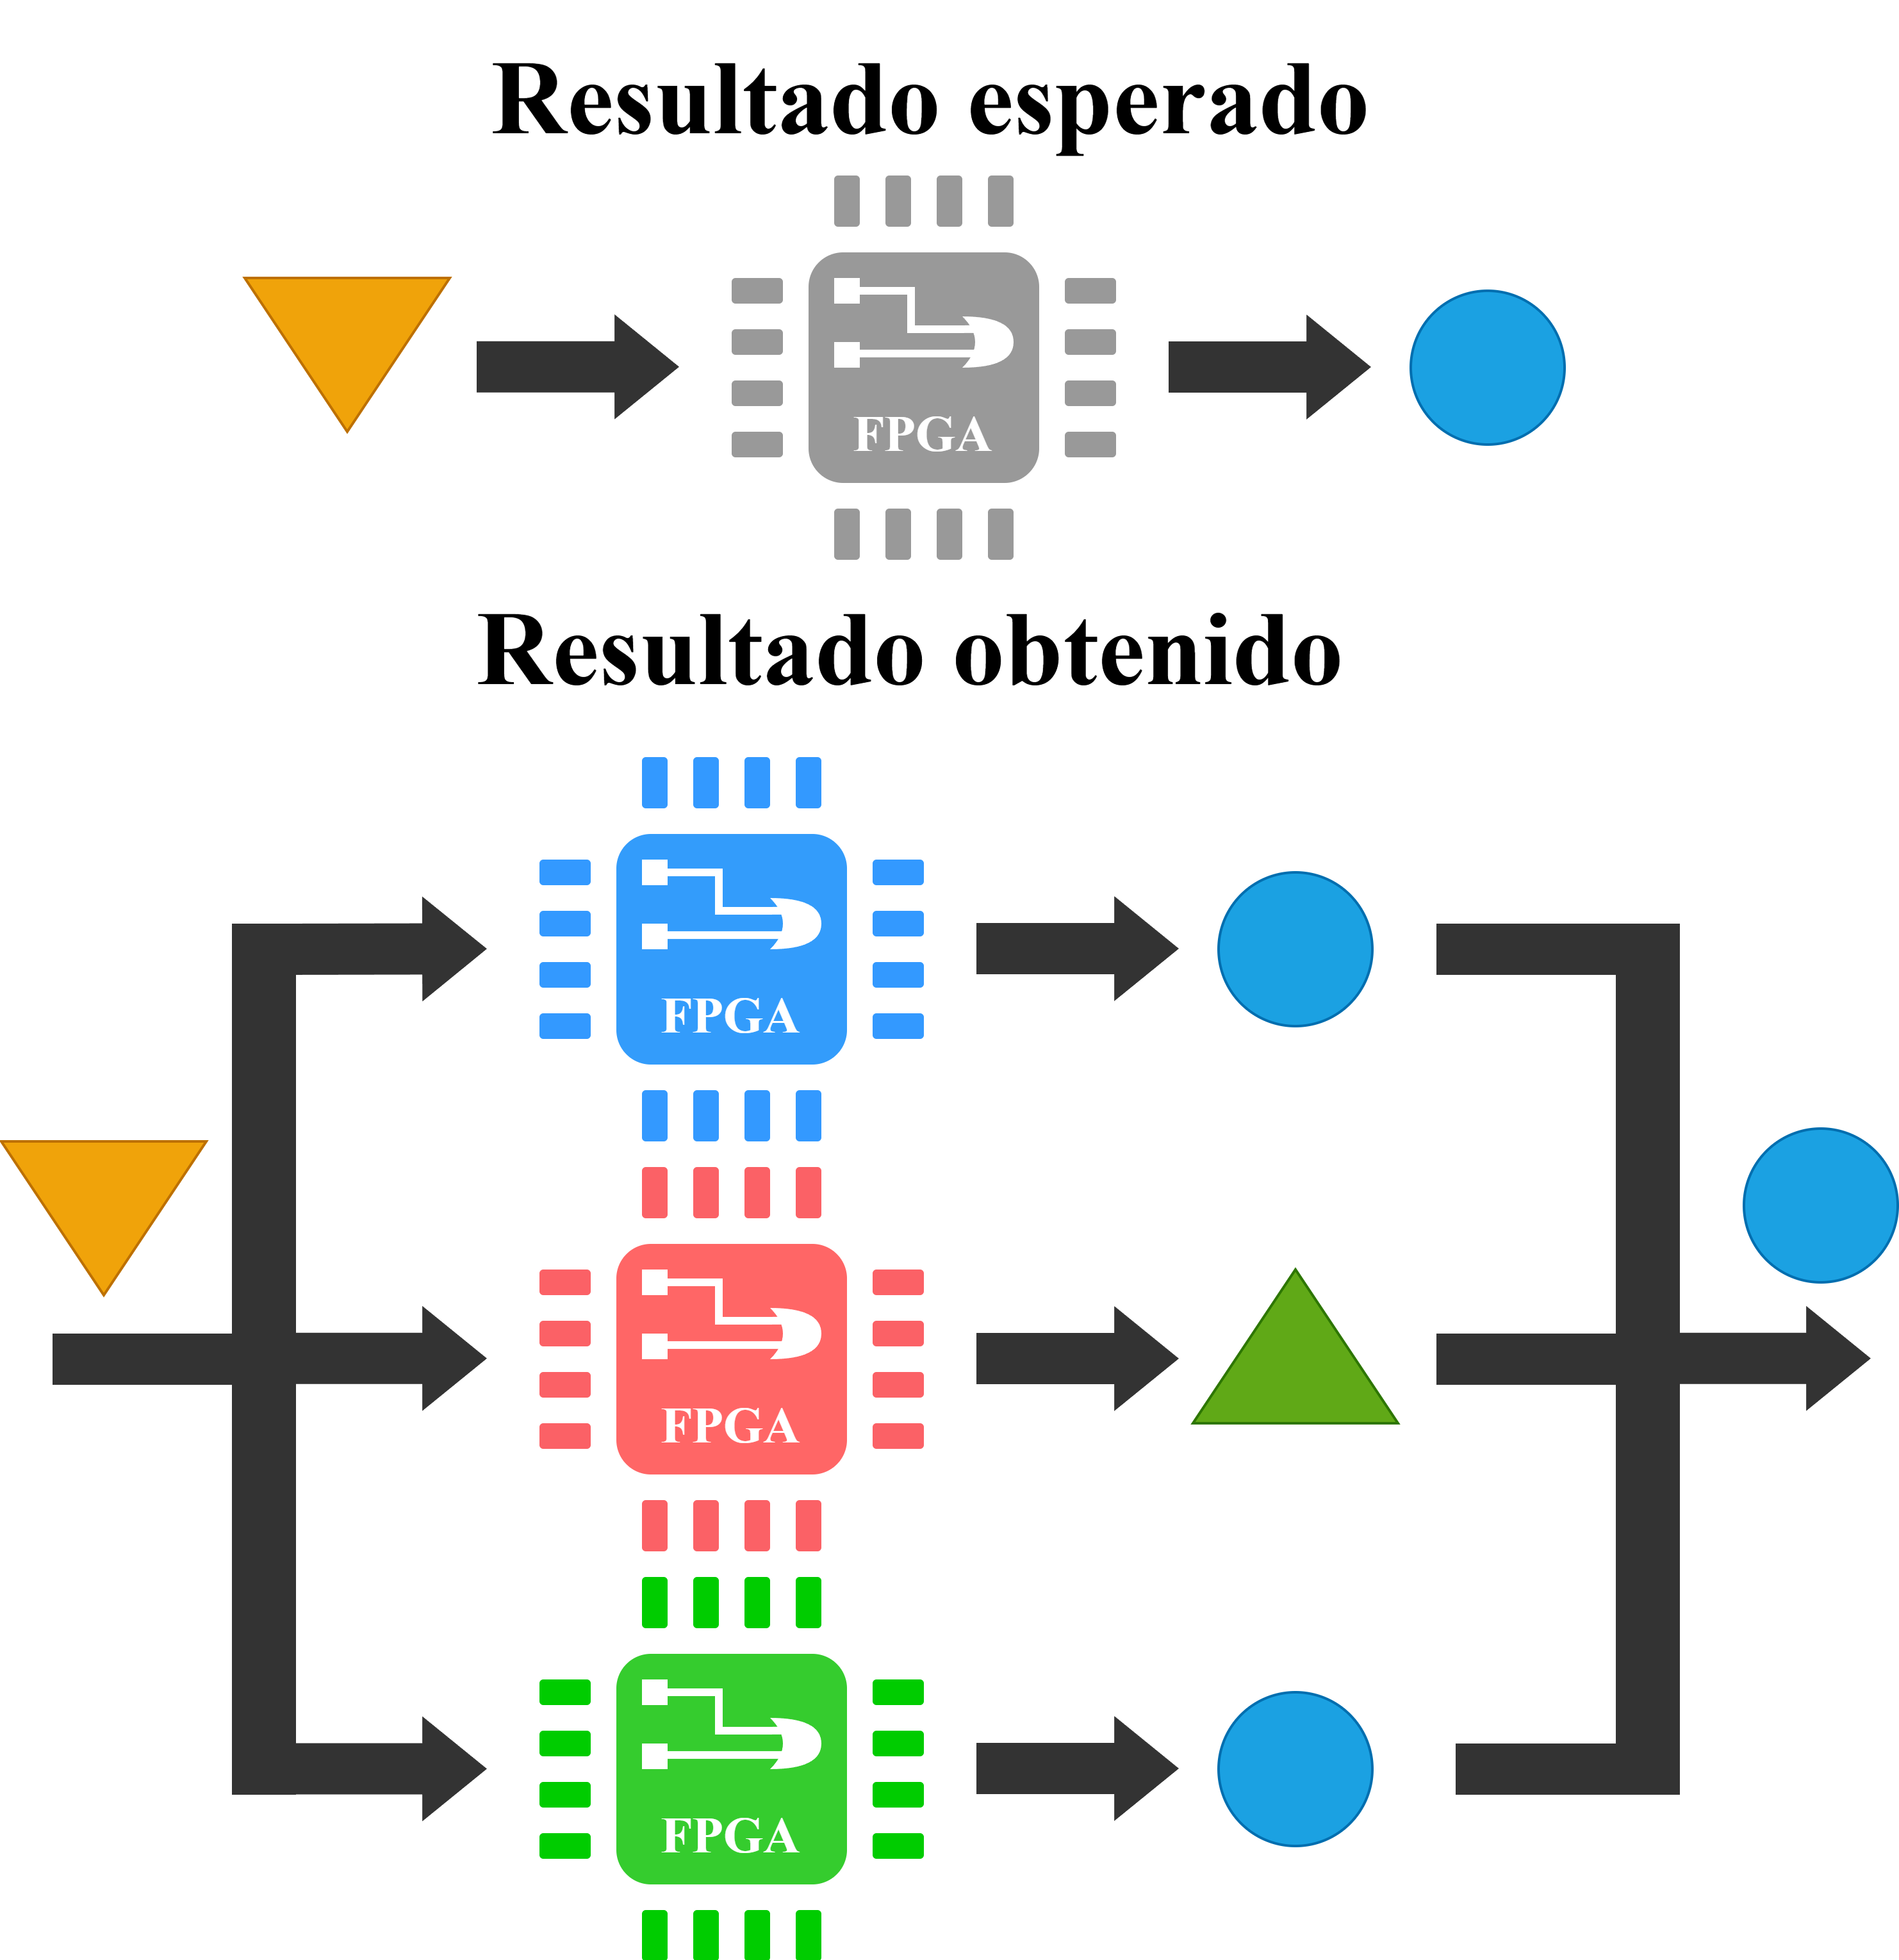
\includegraphics[width=1\textwidth]{Figuras/redundancia.png}
        \centering\caption{Sistema con redundancia 2oo3 y diversidad.}
        \label{fig:redundancia}
    \end{figure}
    
    La tasa de fallas de los sistemas utilizados no puede ser cero, pero debe ser lo mas pequeña posible. Existen fallas de causa común asociadas al fabricante de componentes, defectos eléctricos en los materiales, desperfectos en el software replicados en cada uno de los módulos, etc. Para mitigar las fallas de causa común y robustecer el sistema, se aplica el concepto de diversidad. En el caso de la Figura \ref{fig:redundancia}, esta diversidad está representada en los módulos de diferentes colores: azul, rojo y verde. De esta forma se busca simbolizar que los tres sistemas cumplen la misma función, pero de manera diferente (distintas plataforas y/o distinto lenguaje de programación o incluso diferente equipo de desarrollo). Los tres módulos tendrán, por lo tanto, tasas de falla distintas. Se asume, además, que los módulos pueden tener fallas simultáneas pero de probabilidad mucho mas baja que la tasa de fallas inherente a cada módulo.
    
    De la investigación realizada surge que el 66\% de las empresas utiliza una redundancia 2oo2 o 2oo3 para alcanzar los niveles de seguridad requeridos [REF]. Solo una pequeña porción de las mismas utiliza redundancias 1oo2 [REF] o 2oo4 [REF]. En consecuencia, se puede afirmar que una redundancia 2oo2 o 2oo3 es representativa de los sistemas analizados y puede utilizarse como esquema de partida para un diseño propio.